\chapter{Design}


\begin{figure}[]
\centering
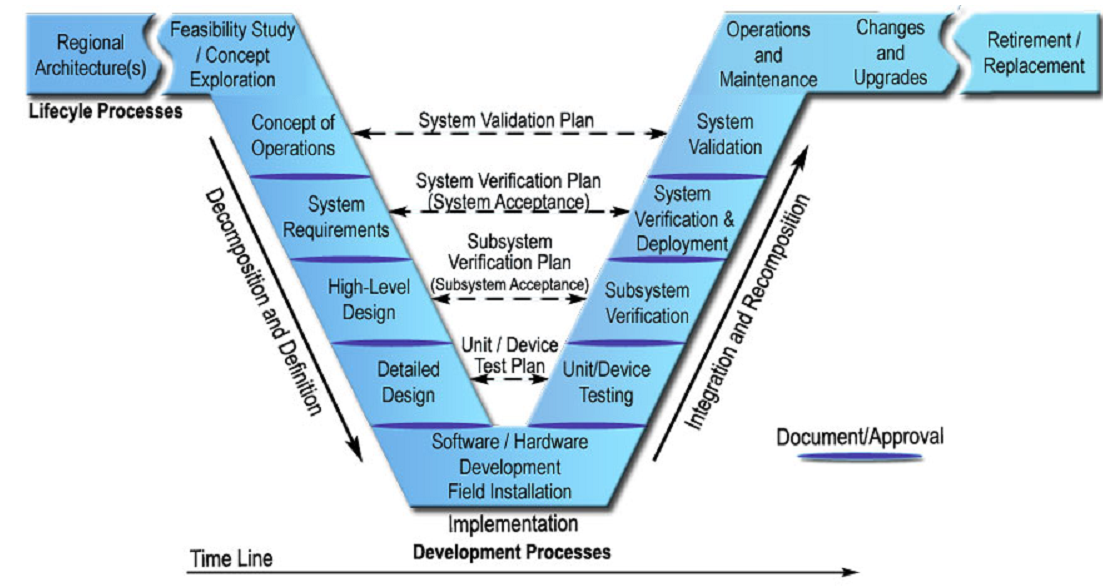
\includegraphics[width=\textwidth]{figures/vee_diagram}
\caption{Vee Diagram}
\label{fig:vee_diagram}
\centering
\end{figure}



\section{Design Context}
This study is within the scope of an undergraduate level approach to both radar and machine learning, with an emphasis on machine learning; the techniques applied herewith are not limited to radar imagery, but attempts should be made to tailor the design to target recognition applications. With development this study should be adaptable to commercial use, and be helpful to people in the radar department who need assistance with radar target classification. Thus the study should develop an easily extensible framework for radar image classification, or at least guidelines to allow others to integrate with the work covered herein.


\section{Feasibility Study / Concept Exploration}
Does the classification of radar imagery lend itself to deep learning techniques, and if so, will the performance be better or worse than na{\"i}ve classification methods? This is the question that best captures the analysis of the study's feasibility.

Consideration of this question needs to include the format of the data entering the system, the ability of the system to process such data, and the effectiveness of the classification of the data.

The data consists of images of between 2916 (54x54) and 37054 (192x193) pixels in size. Each image contains one target, positioned at the centre of the image. This should allow for effective resizing of images to account for size discrepancies. Each pixel in an image constitutes an input. The computational cost of processing the largest image in the set versus the smallest will be at least 12.7 (37054/2916) times more expensive. Initial thoughts were that processing of such images will be made much more feasible if they can be reduced in size to match the smallest images present in the dataset, or at least be made as small as possible while retaining all of the information needed to classify each target. However, the shadow of each radar target often extends outside the 54x54 pixel range, yet could be necessary in classification. Preserving features inherent to each image is more important if the classifier can handle the largest images in a timely fashion. 

Neural networks have a fixed structure; a collection of input neurons feeding their values through a series of hidden neuron layers before arriving at an output layer of neurons equal in size to the number of classes present in the data. The architecture of the network - the choice of number of hidden layers, the number of neurons in each hidden layer, and the number of neurons in the input layer are all subject to change during the development of the system. The training and operation of the system occurs through the adjustment of inter-neuron weights, with the structure of the system remaining constant.

The choice of size of the input layer is crucial; it must remain constant throughout the training and operation of the network. Since each pixel in an image forms of the input layer's neurons, all of the input images must be processed to contain the same number of pixels before any other work on the network's architecture can begin. 

Once the pre-processing of the input images is complete, the structure of the neural network can be decided. This structure shall be changed and prototyped in order to try to find a good corresponding fit for the data. Having too many hidden layers will greatly increase the time taken by the back-propagation algorithm to optimise the weights of the system, and the likelihood of it settling at a local instead of global minimum increases with the complexity of the system. 

The number of neurons in each hidden layer must also be chosen carefully; too many neurons in each layer will result in much longer optimization time (proportional to the increase in the number of inter-neuron weights created). Having too few neurons in a layer can result in the system being unable to extract the features key to classification, and too many neurons may lead to `overfitting' of the training data, leaving the system with no predictive capability (an inability to classify data not present in the set of training instances).


\section{Decomposition and Definition}
This section is devoted to describing the study in terms of its requirements, operation, and implementation. An accompaniment explaining the verification and validity of each subsection will be in the next section.
\subsection{Concept of Operations}
Radar target classification is an inexact science; interpreting a radar image and comparing it to a known case is not as straightforward in all cases as one might expect. Weather conditions, environmental clutter, and image resolution all obscure the target to varying degrees, making intuitive classification ineffective. Computer-based classification through analysis of multiple targets and the application of deep learning techniques should in theory allow distorted images to be classified after the computer is trained to recognise features pertaining to each class. Na{\"i}ve methods of classification lack predictive power - the ability to 'guess' effectively if the target is obscured or unrecognised. Deep learning methods are the solution that this study proposes.

\subsection{User Requirements}\label{sec:user_req}
The success of this report is based on the ability to correctly classify and recognise radar targets taken from the supplied dataset using deep learning techniques. 

The following is required:

\begin{itemize}
	\item Use the MSTAR dataset (Section~\ref{lit:MSTAR})
	\item Develop a na{\"i}ve classifier to use as a benchmark
	\item Use deep learning methodology to develop a classifier 
	\item Indicate how the classifiers can be improved
	\item Comment on the performance of each classifier
	\item Report on the suitability of deep learning for target recognition
\end{itemize}

\subsection{Design Specifications}\label{sec:design_spec}
Expanding upon the user requirements, the following design specifications have been derived:

\subsubsection{The system must be trained on the MSTAR database of radar images}
The images in the MSTAR dataset have undergone a level of pre-processing, making them suitable for rapid prototyping and development of classifiers.

\subsubsection{The system must have a testing accuracy of above 95\%}
Correct identification of radar targets is the aim of this entire report, and as such is the most important performance metric to consider.

\subsubsection{The system must be resistant to noise}
Real-world conditions are not optimal; the classifier must be robust enough to handle the addition of Gaussian white noise to the dataset, without losing more than 1\% classification accuracy.

\subsubsection{The system must have a training time of less than 10 hours}
Training time is taken as being freely available, but any classifier that takes longer than 10 hours to train on the MSTAR dataset will not be worth considering.

\subsubsection{The Nearest Neighbour classifier should be used as a benchmark for classifier comparison}
The NN classifier provides a good example of a na\"ive classifier, and should be beaten by any classifier that is somewhat optimised for the dataset in use. The NN classifier serves as a good benchmark to improve upon, as it gives a lower bound of expected results

\subsubsection{At least two different classifiers should be tested against the Nearest Neighbour classifier}
The chosen classifiers are the K-Nearest Neighbour classifier optimised to fit the dataset, and the Multilayer Perceptron, which satisfies the need for a deep learning classifier.

\subsubsection{Each classifier must be evaluated and compared}
The performance metrics to be used  are training time, classification time, and classification accuracy.

\subsection{High-Level Design}
After analysis of the user requirements, the following areas of design need to be focused on:

\begin{itemize}
	\item Identification/classification
	\item Image Processing/Preparation
	\item Dimensionality Reduction
	\item Na{\"i}ve Classification (Nearest Neighbour as a benchmark)
	\item Deep Learning Classification (Multilayer Perceptron)
	\item Obtaining classifier performance metrics
	\item Classifier comparison
	\item Classifier optimisation
\end{itemize}



\subsection{Detailed Design}
\subsubsection{Image Processing/Preparation}\label{sec:cropping}
The MSTAR dataset is a compilation of image chips, all of which contain a header, as well as magnitude and phase data. The images are between 54x54 and 192x193 pixels in size, which suggests that some form of image processing should be performed to make sure that all images are the same size. The targets in each image chip are centred, suggesting that cropping each image to a size where the target (and its shadow - useful in classification) are left whole, and as much of the surrounding clutter as possible is removed.

An alternate approach is to retain the data inherent in the environmental clutter and pad the smaller images with zeros, keeping all images in the set at the size of the largest image in the set. While this preserves all of the image chip data, processing larger images leads to longer training and classification times.

A compromise is to ensure that all images are the size of the largest image in the set, and somehow reduce the clutter present in each image. Because the targets are substantially brighter than their surroundings, using some form of thresholding (setting values lower than a specified threshold to zero) should prove to be effective in lessening the impact of the clutter, if not completely removing it.

\subsubsection{Dimensionality Reduction}
Each pixel in an image is taken as an feature, forming a feature vector with a length equal to the total number of pixels in the image. The image cropping mentioned in Section \ref{sec:cropping} is very effective at reducing the size of this feature vector. If a 128x128 image is cropped to 64x64, the feature vector's length is reduced by factor of 4. This can be reduced further through the application of dimensionality reduction techniques, such as Principal Component Analysis, Locally-Linear Embedding, Sum of Means and non-linear methods, all of which are outside the scope of this report. As such, each image will be rescaled and padded with zeros to match the size of the largest image in the MSTAR dataset (192x193). This allows every possible feature in each image to be used, while allowing for dimensionality reduction to be implemented at a later stage if desired.

\subsubsection{Nearest Neighbour Design}
\begin{figure}
\centering
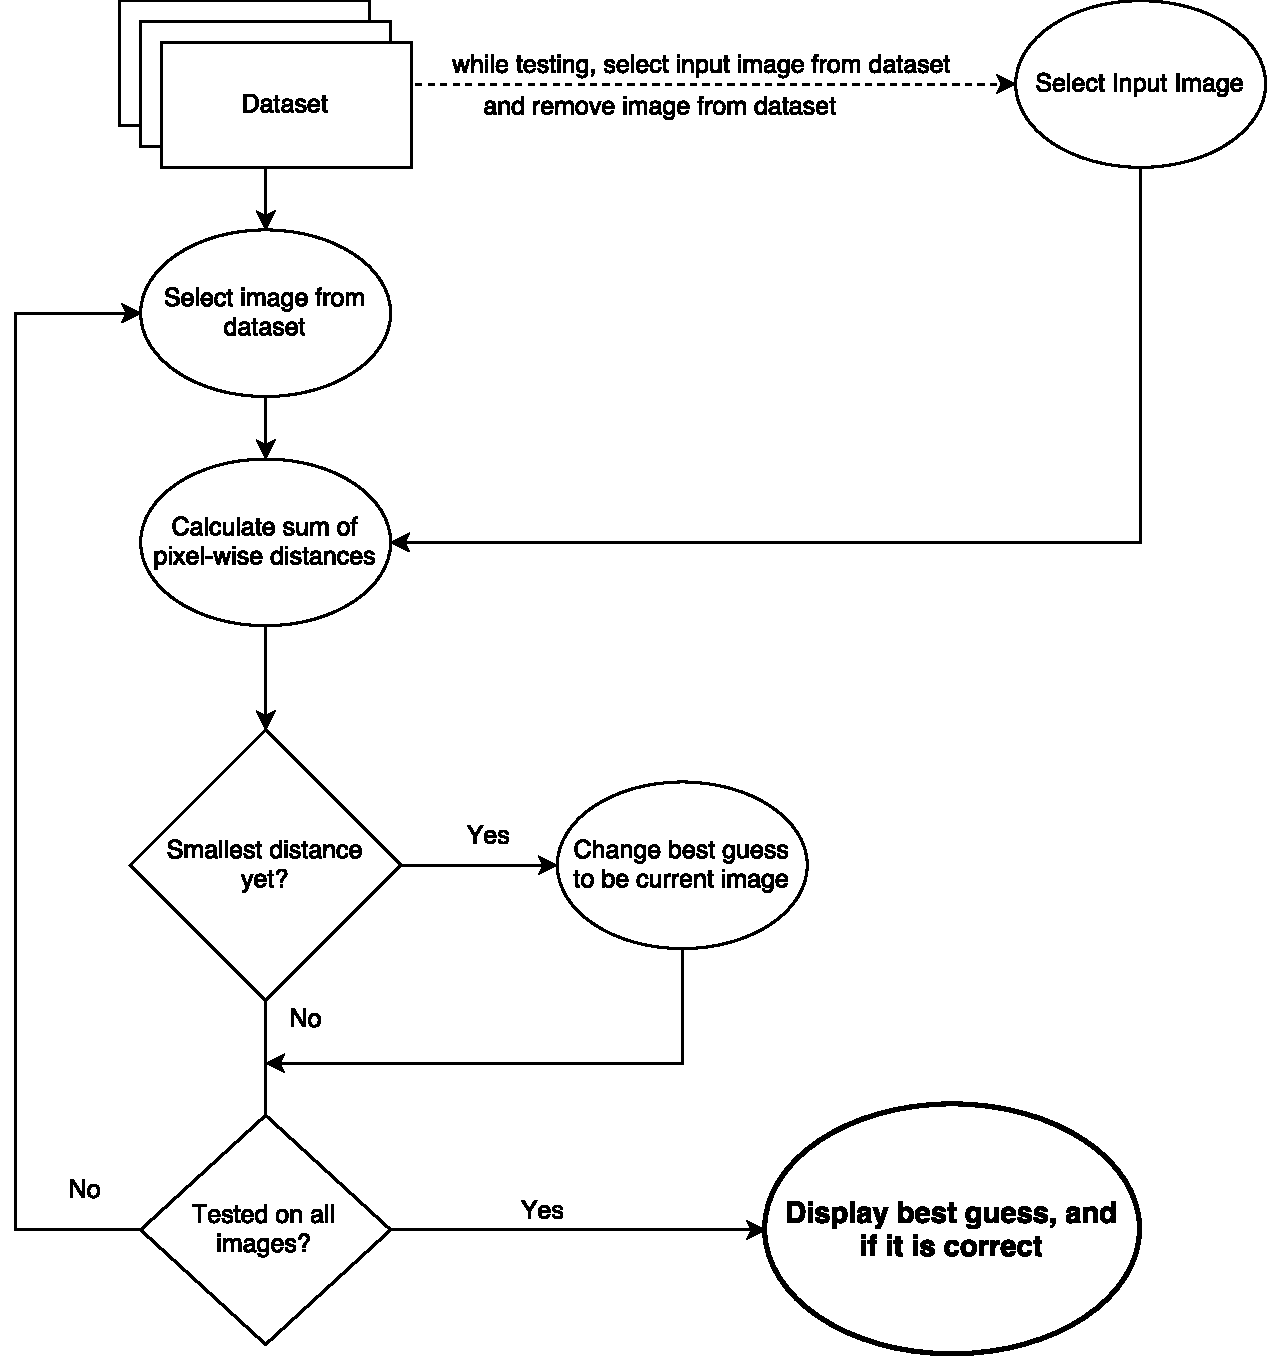
\includegraphics[width=\textwidth]{figures/nearest-neighbour}
\label{fig:nn}
\caption{Nearest Neighbour Classification Flow Diagram}
\centering
\end{figure}

\begin{figure}
	\centering
	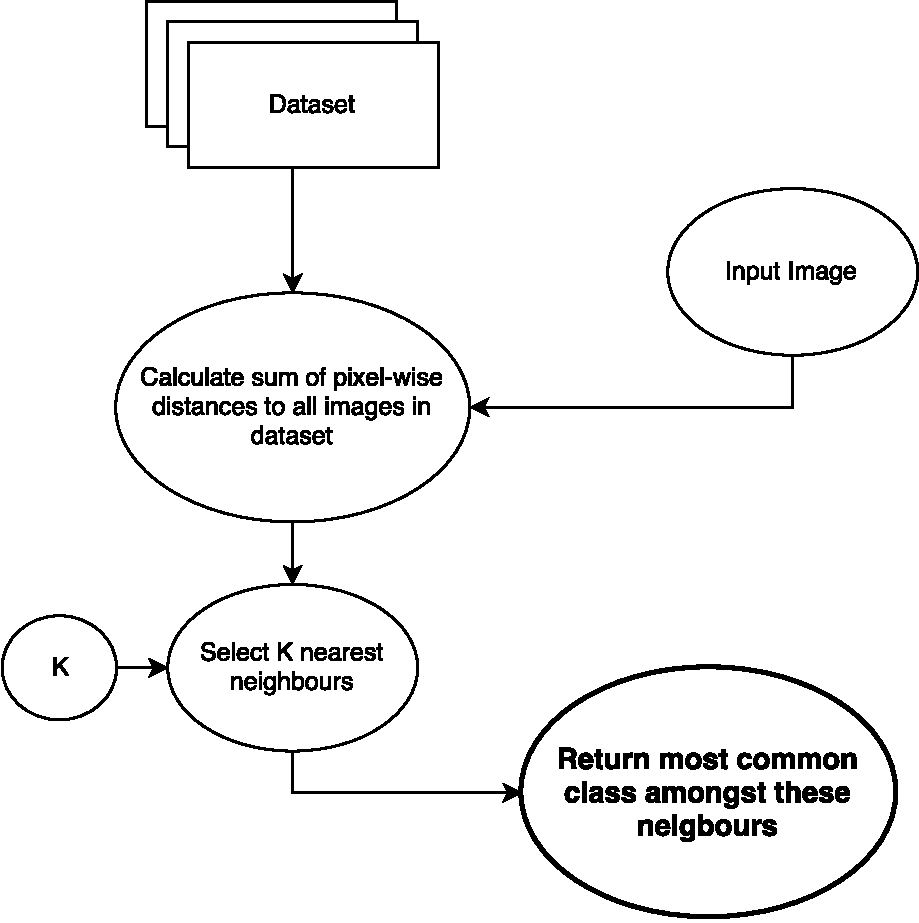
\includegraphics[width=\textwidth]{figures/KNN}
	\label{fig:knn}
	\caption{K-Nearest Neighbour Classification Flow Diagram}
	\centering
\end{figure}

\begin{figure}
	\centering
	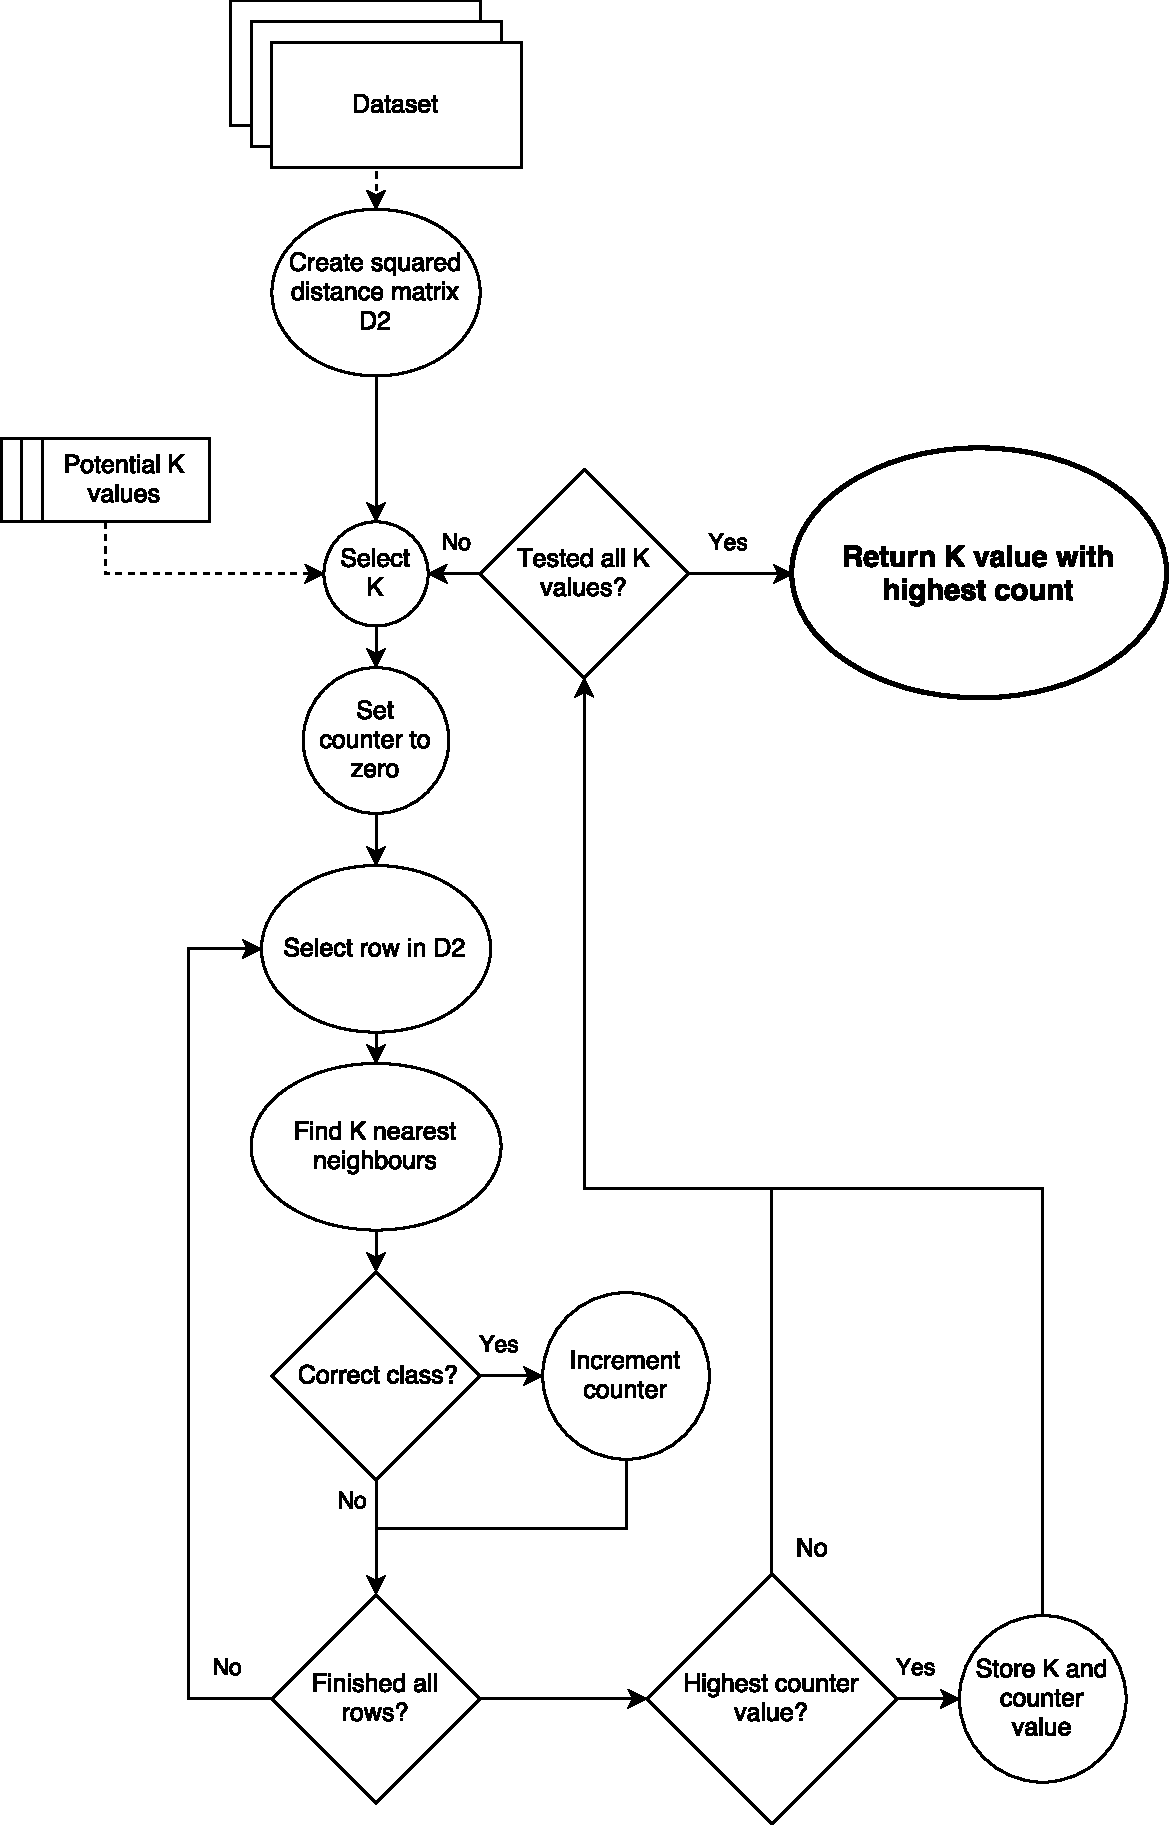
\includegraphics[width=\textwidth]{figures/k_values}
	\label{fig:knn_values}
	\caption{K-Nearest Neighbour Optimising for `K' Flow Diagram}
	\centering
\end{figure}



The high-level design is shown in Figure~\ref{fig:nn}. Its principles of operation are covered in Section~\ref{lit:nn}. To implement this classifier, the following is needed:

\begin{itemize}
	\item Access to the dataset
	\item A choice of input image
	\item A method to calculate and sum the pixel-wise distances
	\item A variable storing the smallest distance and tentative classification
	\item A method displaying the chosen class and whether or not it is correct
\end{itemize}

\subsubsection{K-Nearest Neighbour Design}
While similar to the Nearest Neigbour design, 
KNN introduces its own complexities, most notably when optimising for K. The high-level design is shown in Figure~\ref{fig:knn}, its principles of operation are covered in Section~\ref{lit:knn}. The method of finding the best K value for a given dataset is shown in Figure~\ref{fig:knn_values}.

\subsubsection{Multilayer Perceptron Design}

Implementation of a multilayer perceptron in software can be divided into discrete sections as follows:
\begin{itemize}
	\item Implement a wrapper class for the classifier
	\item Develop a logistic regression layer class to use at the output
	\item Develop an extensible hidden layer class
	\item Collate the important details of each layer in the wrapper class
	\item Implement a test method
\end{itemize}

\section{Software Design}
\subsection{Guidelines}
Developing the software for this report is done with the following objectives in mind:
\begin{itemize}
	\item Comment code clearly
	\item Use logical code structure and layout
	\item Use Python as the chosen programming language
	\item Use Theano module for deep learning calculations
	\item Code self-contained classifier classes
	\item Difficult to generate data should be saved for future use
	\item Code reusable, adaptable methods
	\item Make performance metrics readily available
	\item Test while developing
	\item Provide a comprehensive `README' for new users
	\item The code must be available online at ~\href{http://github.com/roansong}{github.com/roansong}.
\end{itemize}

\subsection{Testing and Optimisation}
\subsubsection{Testing}
Each classifier has unique testing methods, but the performance metrics on which there are compared are the same. The metrics we are interested in are:
\begin{itemize}
	\item Time taken to classify a single instance
	\item Time taken to train the classifier
	\item Classification accuracy of the classifier
\end{itemize}

\subsubsection{Optimisation}
Where possible, each classifier must be optimised to improve its classification accuracy and classification time. Training time is considered acceptable if it is less than ten hours, as specified in Section~\ref{sec:user_req}. \\

The K-Nearest Neighbour classifier must be optimised to find the value of K that best fits the dataset.
The Multilayer Perceptron must be optimised for its learning rate, L1 regularisation, L2 regularisation, hidden layer size, and number of hidden layers.

\subsubsection{Inline Testing}
While implementing the software for this report, I ran into some early issues that resulted from insufficient planning. After taking a step back, it was decided that more steady progress would be made by implementing rigorous inline testing, i.e. incrementally testing the code after every slight modification, instead of only testing after the addition of a major feature and then trying to iron out any latent bugs. This approach leads to much simpler debugging.


\section{Software Implementation}
The implementation of the classifiers and techniques discussed in this report will be covered in this section. 



\subsubsection{Image Pre-processing}

In a process outlined in Figure~\ref{fig:multi_input}, the input image is converted to an array of unsigned 8-bit integers (ranging from 0 to 255). The elements of the array are `normalised' by subtracting the mean of the array from each and then dividing each element by the standard deviation of the array. This ensures that the processed values lie centred around zero, and mostly between -1 and 1. Unsigned integers do not provide enough precision to represent this data, so 32-bit floating point numbers (floats) are used. The code for normalisation is shown in Listing~\ref{list:normalise}.

\begin{lstlisting}[language=Python, caption=Normalisation method, captionpos=b, label={list:normalise}]
def normalise(vector):
"""
Normalises a vector so that most of its values lie between -1 and 1
returns the vector mentioned above
vector --- the vector to be normalised (type: numpy array)
"""
return (vector - vector.mean(axis=0))/(vector.std(axis=0))
\end{lstlisting}

Two additional methods of processing are made available: thresholding and noise addition. Thresholding is done before normalisation. For each image, pixels with values below the median value of the image are set to zero. This eliminates some of the noisy `clutter' present in radar imagery. Noise addition is used to simulate real-world conditions by adding Gaussian noise to the image after normalisation to somewhat obscure the radar signal. The implementations of thresholding and noise addition are shown in Listings~\ref{list:thresholding} and~\ref{list:noise} respectively. The complete code is shown in Appendix~\ref{list:get_images}


\begin{lstlisting}[language=Python, caption=Thresholding, captionpos=b, label={list:thresholding}]
if(threshold):
below_thresh = image < numpy.mean(image)
image[below_thresh] = 0
\end{lstlisting}

\begin{lstlisting}[language=Python, caption=Adding noise to an image, captionpos=b, label={list:noise}]
if(noise):
image += numpy.random.normal(0,1,image.shape)
\end{lstlisting}


 

\subsubsection{Allocation of Data}

Three different sets of data are needed to train a classifier. The training set, validation set, and testing set. Each set contains instances of data (in this case image vectors) and targets denoting the class each instance belongs to. Each set is filled with random images from the original dataset without replacement, with the size of the three sets being determined by a set of three numbers. The numbers do not have to correspond exactly to the number of images in each set - they represent ratios between the sizes. The code to generate the three sets, as well as a tuple of indices showing which instances from the original dataset are in each set is shown in Appendix~\ref{list:gen_sets}.

\subsubsection{K-Nearest Neighbours}\label{sec:best_k}
Developing a standalone Nearest Neighbour classifier and a separate K-Nearest Neighbour classifier is redundant; the NN can be obtained by setting K equal to 1 in the KNN. Only KNN needs to be implemented.

KNN operates by loading a dataset of input instances and targets, and calculating the squared distances between the input instance and every instance in the dataset. Each distance result is appended to a list. After every distance has been calculated, the list is sorted in ascending order, and the K lowest instances are taken. It is important to keep track of the target output associated with each input. These instances with the smallest squared distances are the `neighbours' from which KNN derives its name. The most common class amongst the neighbours is taken as the predicted class. The ratio between the number of neighbours in agreement and K can be used to give a measure of confidence in the prediction.

To optimize K for the dataset, a different approach must be taken. It is inefficient to test every instance in the dataset against every other instance for every possible value of K. Instead, these distances are calculated only once. A squared distance array (D2) is formed by taking every instance in turn and calculating its distance to every other instance, with the knowledge that the distance from an instance A to instance B will be the same as from B to A. This halves the number of calculations necessary to calculate D2. D2 is symmetric along its diagonal, and all of its diagonals are equal to zero. This is because the distance from any instance to itself will always be zero. \\

Each row in D2 provides the squared distances between the instance corresponding to that row and every other instance in the data set. Sorting these distances in ascending order for every row gives the nearest neighbours to each instance. Removing the first instance in each sorted row removes the self-contribution factor of an instance to itself. Chosen values of K can be tested much more efficiently, going row by row and taking the first K instances, seeing if the majority of those K neighbours predicts the correct output, and tallying up a score for each value of K. The value of K with the highest score once every row has been visited is the value of K best optimised for the dataset. The complete KNN code is shown in Appendix~\ref{list:knn}.

\subsubsection{The Multilayer Perceptron}

Once each pixel has been processed, they can be sent to the input layer of the neural network, with each pixel representing a neuron as shown in Figure~\ref{fig:multi_input}.
 
Each of these input layer neurons has a random weight applied, and is then fed into the neurons that form the first hidden layer. Every neuron in the input layer contributes to every neuron in the next layer. At each neuron in the first hidden layer, the `net' value is formed by summing all of the values present at its input (i.e. all the weighted values passed along from the input layer). An activation function is applied to this net value to compress the range of values. There are many different activation functions that can be used, and for this study I narrowed down the choice to either the logistic function $ \frac{1}{1 + e^{-net}} $ or the hyperbolic tangent function $\frac{e^{net} - e^{-net}}{e^{net} + e^{-net}} $. The logistic function produces an output between 0 and 1, while the hyperbolic tangent function's output is between -1 and 1. I decided to use the hyperbolic tangent function, because the logistic function has a tendency to incur long training times if its values lie very close to 0, while the hyperbolic tangent function tends to move towards its extreme values more quickly.  

The activation function, when applied to the net of the neuron, becomes the output of the neuron, feeding through to every neuron in the next layer with weights applied, repeating the same process until the output layer. This is shown in Figure~\ref{fig:multi_neuron} and more closely in Figure~\ref{fig:multi_neuron_close}. 
 
 \begin{figure}[!h]
 	\centering
 	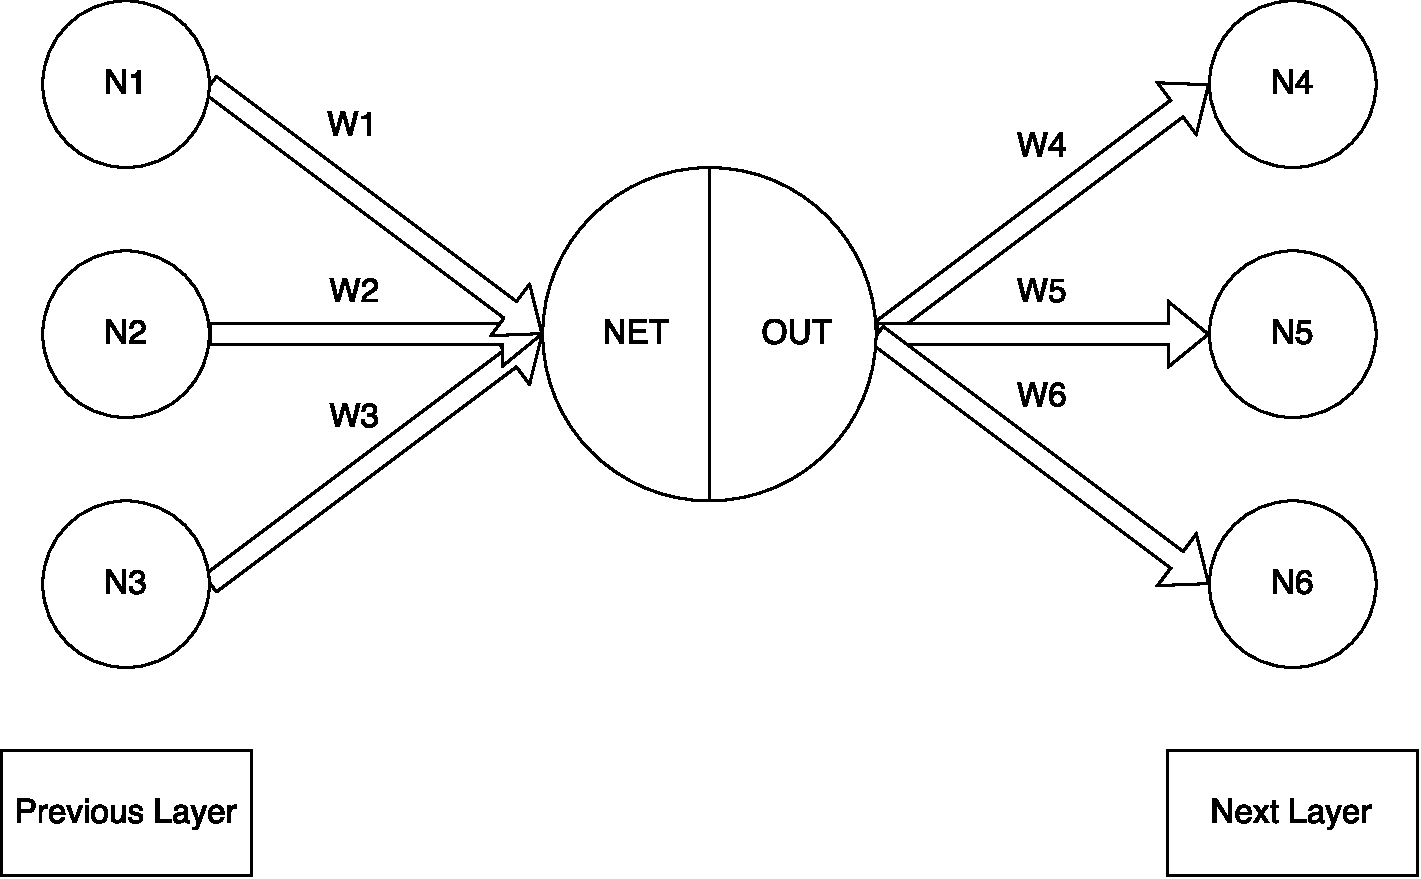
\includegraphics[width=\textwidth]{figures/multilayer_perceptron_neuron}
 	\centering
 	\caption{A Neuron in the Network}
 	\label{fig:multi_neuron}
 \end{figure}

\begin{figure}[!h]
	\centering
	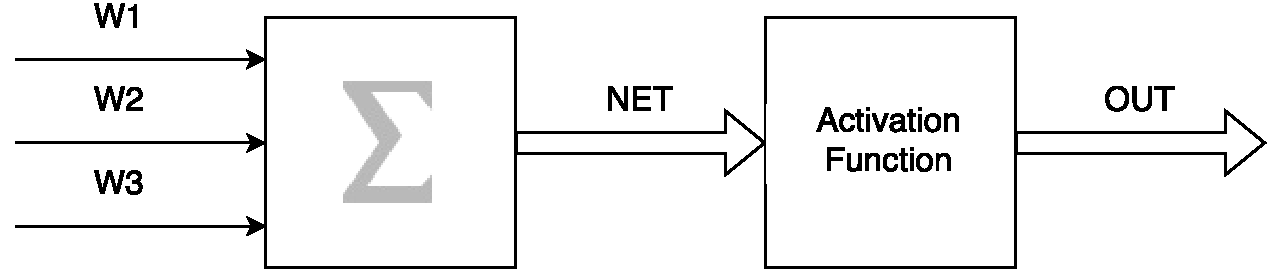
\includegraphics[width=\textwidth]{figures/multilayer_perceptron_neuron2}
	\centering
	\caption{The Internal Workings of a Neuron}
	\label{fig:multi_neuron_close}
\end{figure}
 
 
The output layer has as many neurons as there are classes. The output layer is a logistic regression layer, which has a softmax function applied to its outputs. This results in outputs that sum to 1, with larger values being strongly emphasised. This correlates nicely with the one-hot vectors used to label classes\cite{dunne1997pairing}. The neuron with the highest value is taken to be the network's prediction. An example output would be:
 \[ [0.25, 0.2, 0.1, 0.05, 0.4] \] 
There are five classes, and the fifth class has the highest value, thus the neural network has classified the input as belonging to that fifth class. Given that the maximum possible value for an output would be 1, 0.9 would show a large confidence in the classification. A value close to 0 shows strong disagreement, while 0.3 would show moderately low confidence.
 
To train the network, stochastic gradient descent is used, as described in Section~\ref{lit:grad_desc}. The gradient of the cost function with respect to the weights and biases of each layer is calculated and the weights and biases are updated proportionally to the learning rate. This is shown in Listing~\ref{list:grad_desc}, and is easily achieved through the use of Theano (covered in Section~\ref{lit:theano}).

\begin{lstlisting}[language=Python, caption=Implementing Gradient Descent, captionpos=b, label={list:grad_desc}]
gradients = [T.grad(cost,param) for param in self.parameters]
updates = [(param, param - learning_rate*gparam) for param, gparam in zip(parameters,gradients)]
\end{lstlisting}


\subsubsection{Training and Testing}
The first step is to get to grips with the data - processing the data set in a way that makes sense to use, and allows different classification methods to be implemented easily on it.

The MSTAR dataset contains eight different targets. The dataset is sorted by depression angle, and by `scene'. All of the targets have data corresponding to  15\degree~and 17\degree~elevation angles, for a total of 4459 images. The MSTAR dataset stores the information of each target in a header section of each file. This is inconvenient when reading in image files directly, so the header is discarded and images are classed according to their file extension. The file extensions and the classes they correspond to can be found in Table~\ref{tab:input_data}. To simplify classification, a variant of a one-hot vector denoting the classes is attached to each target. The vector consists of a series of numbers, equal in length to the number of classes in the dataset. A `1' denotes that the instance is a member of the class corresponding to that entry in the vector, and the rest of the numbers are 0, showing that the instance is not in those classes. A file is created listing all of the filenames to be tested during the run of the algorithm. An example file with ten entries and two classes would look as follows:\\

\begin{center}
	\begin{tabular}{c}
		HB03333.003.tiff 1 0 \\
		HB03334.003.tiff 1 0 \\
		HB03335.003.tiff 1 0 \\
		HB03337.003.tiff 1 0 \\
		HB03338.003.tiff 1 0 \\
		HB14931.025.tiff 0 1 \\
		HB14932.025.tiff 0 1 \\
		HB14933.025.tiff 0 1 \\
		HB14934.025.tiff 0 1 \\
		HB14935.025.tiff 0 1 \\
	\end{tabular}
\end{center}

This information is used to form the target set that corresponds to every set of instances.

\subsection{K-Nearest Neighbours}
The KNN is provided with the training, validation and testing datasets. Because KNN undergoes no validation phase, the validation set is concatenated to the training set to provide extra training data. The best value of K is obtained as detailed in Section~\ref{sec:best_k}. This value of K is then used to run every instance in the test set against all the images in the training set. This procedure is timed, and represents the training time metric of the classifier. The number of correct predictions is tallied and is used to calculate the classification accuracy. The time taken to classify a single instance against the dataset is taken as the classification time.

\subsection{Multilayer Perceptron}
Training a Multilayer Perceptron is more complex than training the KNN. Training the MLP revolves around minimising the loss function of the classifier, defined by the negative log likelihood $loss$ of the predicted output to the target output and the L1 and L2 norms of the network's weights, adjusted by the L1 and L2 regularisation factors $a$ and $b$. These factors sum to form the cost of the classifier, as shown below:

\[cost = loss + a*L1 + b*L2\]

This cost is minimised through training. It is important to note that the regularisation of the inter-neuron weights is thought to improve the classification accuracy, with smaller weights providing more general predictive capabilities. Minimising the cost function entails balancing loss and weight minimisation to prevent over-fitting of the training dataset.

Using the Theano module, the symbolic gradient of the cost with respect to each parameter that contributes to it is calculated, as shown in Listing~\ref{list:grad_desc}. \\

Before training can commence, the parameters of the training session need to be chosen. The number of epochs specifies how many iterations over the dataset are to be done before returning. The batch size determines the number of batches and how many instances are in each batch when implementing stochastic gradient descent. Early stopping parameters are chosen, such as the option to stop training once testing error is zero, and the `patience' of the training. The patience defines the number of instances to train on without improvement before stopping early. If the results obtained within this patience interval demonstrate improvement, the patience interval is extended. Improvement is measured by seeing if a new value falls under a threshold deemed significant (taken as 99.9\% as default in this implementation).

During training, the error of the classifier is averaged over each training batch and the parameters of the system are adjusted in proportion to the learning rate. After training on every training batch once, the classifier is trained on the validation batches, averaging the errors returned for each batch. Note that the error is not the same as the cost - error is the zero-one loss between the predicted output and the target output, and is shown in Listing~\ref{list:error}.

\begin{lstlisting}[language=Python, caption=Calculating Zero-one Error, captionpos=b, label={list:error}]
    import theano.Tensor as T
    def errors(self,target):
		"""
		Returns the average error between the predicted class and the target class
		target --- correct output
		T.neq is the logical inequality function
		"""
		return T.mean(T.neq(self.predicted_class,target))        
\end{lstlisting}

If the improvement seen in the validation batches is significant, the patience value is increased. During validation the model parameters are also updated via stochastic gradient descent.

After validation, the test error or `test score' is calculated by testing the model on data not in the training or validation sets. The error is the average of the zero-one errors over all test cases. If the test score has improved, the state of the model is saved by storing the inter-neuron weights on disk. If previously specified, if the training error is equal to zero, the training can stop, otherwise the classifier continues to train. There is a benefit to continuing in that the classifier cost can be reduced further, at the risk of over-fitting.

Once training is complete, the performance metrics of the classifier are stored. The training procedure is timed, a single instance is tested and timed to find the single-class classification time, and the classification accuracy of the classifier on the test set is noted.

Other metrics specific to the MLP are also stored; the shape of the classifier (how many hidden layers and their sizes), the best test score, final validation error, and final training error, as well as the final cost of the classifier.

\begin{figure}[!h]
	
	\centering
	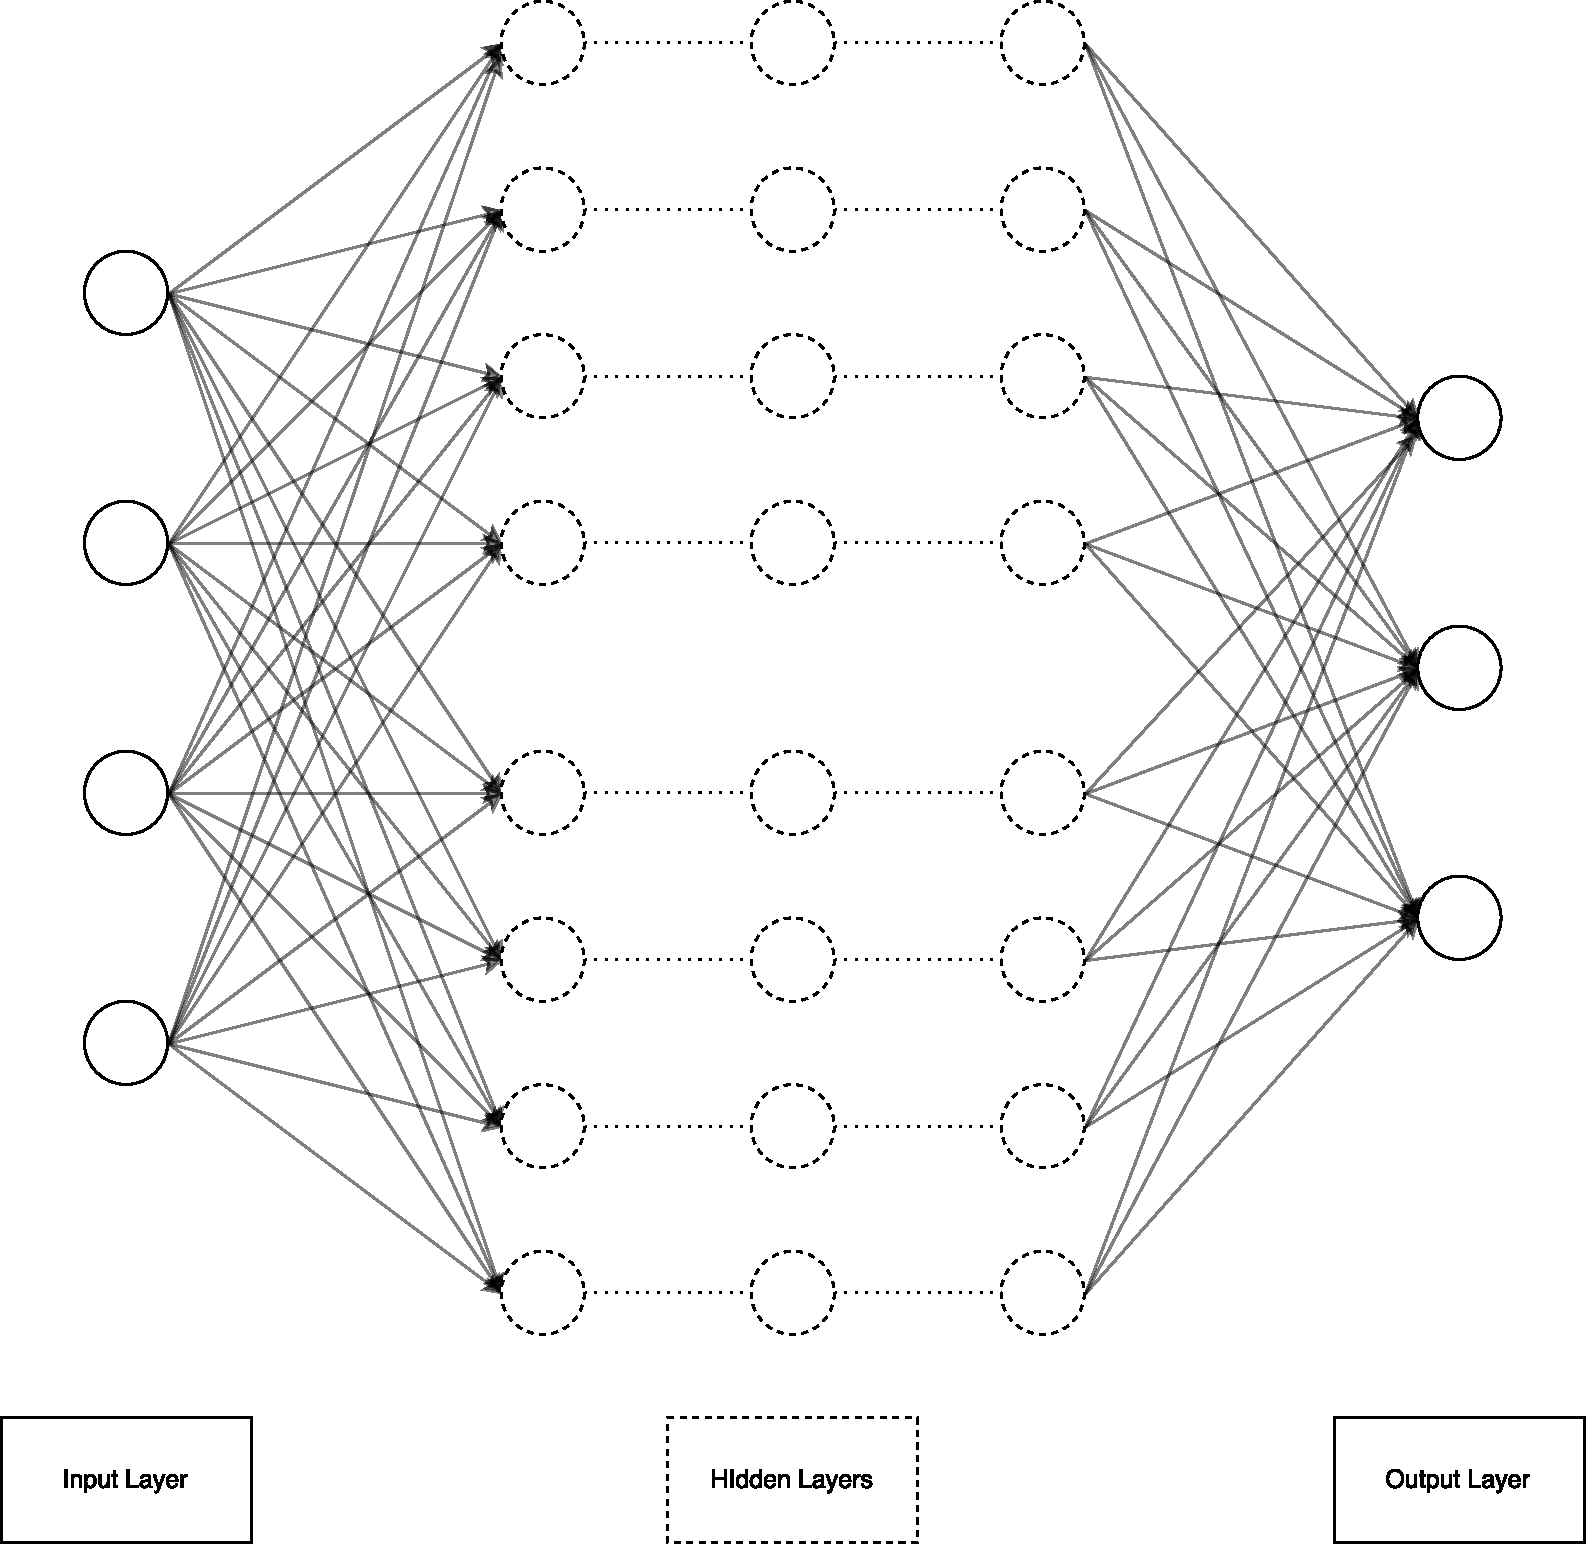
\includegraphics[width=\textwidth]{figures/multilayer_perceptron}
	\centering
	\caption{Multilayer Perceptron Overview}
	\label{fig:multi}
\end{figure}


\begin{figure}[!h]
	
	\centering
	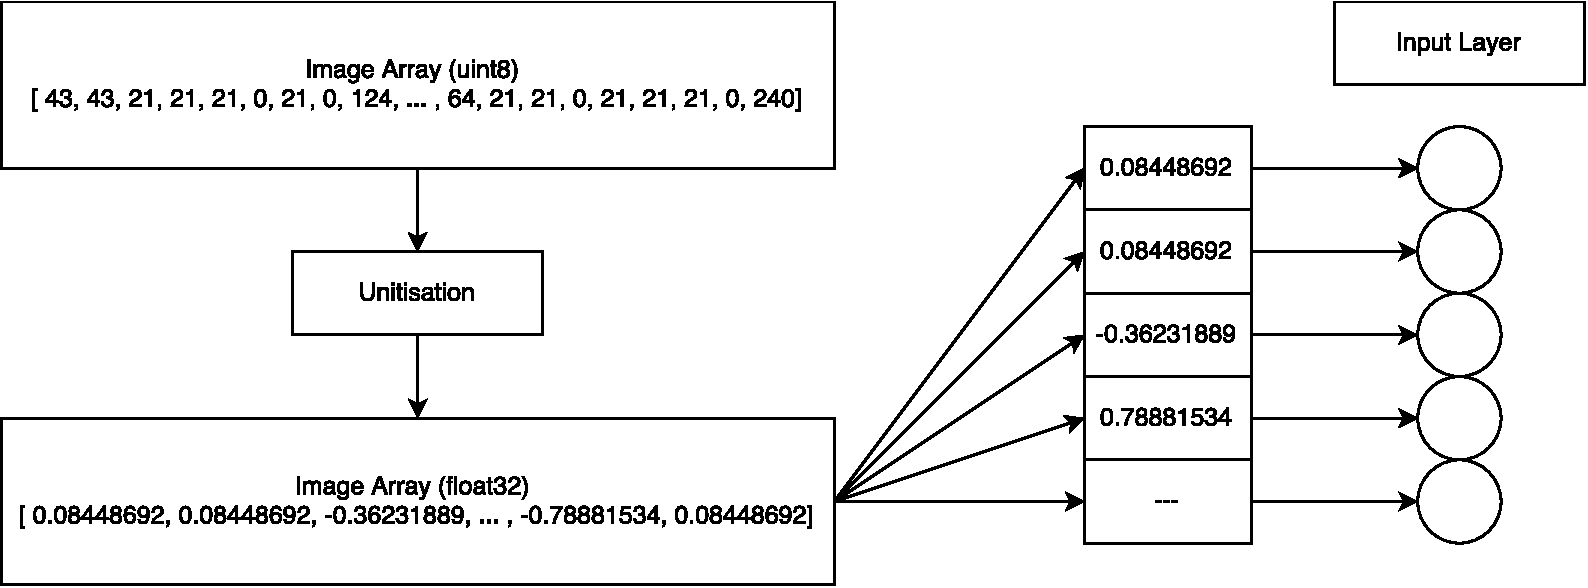
\includegraphics[width=\textwidth]{figures/multilayer_perceptron_input}
	\centering
	\caption{Multilayer Perceptron Input Layer}
	\label{fig:multi_input}
\end{figure}


\subsubsection{Testing During Development}
The simplest way to find a classifier's efficacy is to test it on a wide variety of classes and on as many test instances as possible. To provide interim results, during the iterative phase of classifier development, only a subset of the dataset's images are used. This compromises the final accuracy of the classifier (it may perform differently on the full dataset), but brings with it the ability to test and train classifiers more quickly, due to the lower computational overheads. During the development this testing method allows for simple decisions regarding the direction of classifier implementation or optimisation to be made. In process of verifying the classifiers, the full dataset must be used to give an accurate picture of the classifier's performance and real-world implementation. 

\section{Integration and Recomposition}

\subsection{Subsystem Verification}
The chosen method for verifying a classifier's efficacy once it is considered to be sufficiently optimised is simple; The classifier is tested on the dataset with a number of test instances as in Section~\ref{lit:loocv}. For the KNN, fully testing it entails removing one instance from the dataset, training the classifier on the remaining points, and using the removed instance as a test case. Once this has been done, the instance is replaced, another is taken, and the process is repeated until every instance in the dataset has been tested. The system's performance is based on the number of correct classifications made during the process. This is known as Leave-One-Out Cross Validation (LOOCV).

\subsection{System Verification and Deployment}
To confirm the results of each classifier, it is important to have a set of training instances on which the system can be trained. The system is then tested on another set of points whose classes are known. Once this has been tested and confirmed to have a desirable level of classification accuracy, the system will be ready for testing on previously unseen, real-world cases. 

This is accomplished by dividing a set of known data points into a training set, a validation set, and a testing set. For example: 80\% of the data points will be used to train the system, 10\% to validate the model, which will then be tested on the remaining 10\%. The process of cross-validation entails selecting a different training/test split each time (either systematically or at random) and performing the process again. This concept can be extended to where the system is trained on all but one of the instances and then tested against it, which is known as LOOCV ("Leave One Out" Cross-Validation). The system is tweaked until it reaches the level of classification required. Cross-Validation is an important tool for eliminating "overfitting" of the system to the training data. Mixing up the training and test cases ensures that the classifier is left with some ability to generalise, and not just repeat what it has been shown.

\subsection{System Validation}
If the objectives of the report have been accomplished, the system will be considered valid. The results found during this report have to be collated and analysed within the context of its requirements. This goes beyond confirming the individual results of each classifier and seeing if implementing deep learning techniques are indeed the `smart choice' in the task of radar target recognition. 

\subsection{Operations and Maintenance}

Considering the real-world application of a target recognition system, it should meet certain criteria to ensure ease of use and compatibility with various datasets. Providing adequate documentation to support the system is key. 

The documentation must detail:
\begin{itemize}
	\item The operating procedure of the system
	\item The expected input to the system (dataset and individual instance)
	\item The output format of the system (predicted class and performance metrics)
	\item Comprehensive troubleshooting (outside the scope of this report)
\end{itemize}

\subsection{Changes and Upgrades}

If the system is required to be maintained and expand its scope (by incorporating more, larger, and more complex images into its dataset), the input data will have to undergo pre-processing that is not currently implemented into the system, such as intelligent dimensionality reduction. The system may have to restructure some of its key classification methods and re-optimise hyper-parameters. 

A classification method to consider for real-world use is a Convolutional Neural Network, as it can classify targets without the need for the target to be centered (as in the MSTAR dataset). This would be more suited to real-world applications, although the classification time is longer. This is not trivial, and lies outside the scope of this report.













